% !TEX root=../pldi2019.tex



\section{Semantics}
\label{sec:semantics}

% In the previous section we introduced our workflow calculus,
% and described semantics of each construct intuitively.
In this section we will formalise the intuition of each language construct described above.
To do this,
we need to take into account the way our calculus is structured.

Firstly,
we have seen our calculus is embedded into a simply typed $\lambda$-calculus.
This requires us to specify how the host language \emph{evaluates} its expressions,
and how it handles our domain language.

Secondly,
we have seen two ways to decide how to proceed from one task to another:
internally by the system itself, or externally by the user.
This means we need two additional semantics:
one to specify the internal \emph{normalisation} of tasks,
and another to define the \emph{interaction} with the end user.

One could choose to merge evaluation and normalisation.
We do not do so,
because it would pollute the semantics of the host language with workflow specific semantics.
By lifting normalisation to an additional layer,
tasks will be ordinary values for the host language.

The three main layers of semantics are evaluation, normalisation, and interaction.
Together with \emph{observations} we will discuss these smantics in the subsections to come.
\Autoref{fig:semantic-functions} shows the relation between these semantics.
It also shows that we will make use of two \emph{helper semantics}.
Normalisation will make use of \emph{striding} semantics,
and interaction makes use of \emph{handling} semantics.

\begin{figure}[h]
  \centering
  \includegraphics[width=\columnwidth,page=5]{figures/drawings-crop.pdf}
  \caption{
    Semantic functions defined in this report and their relation.
  }
  \label{fig:semantic-functions}
\end{figure}

We use the convention that downward arrows represent big-step semantics.
Rightward arrows are small-step semantics.
Also, double arrows make use of single arrows,
e.g, the double down arrow $\normalise$ \emph{uses} the single down arrow $\evaluate$.



\subsection{Evaluating expressions}
\label{sec:evaluation}

To express evaluation,
we use the big step semantics of our host language.
Turning an expression $e$ in state $s$ into a value $v$ in state $s'$ is denoted by $\RelationE$.
To ease reasoning about references,
we choose our host language to be \emph{eagerly} evaluated.

\Autoref{fig:value-grammar} shows values with respect to the evaluation semantics.
% Regarding our base language, lambda abstractions are values, as are all constants.
Each \emph{pretask} $p$ is accompanied by a corresponding \emph{task} $t$,
which are also values with respect to evaluation.
Only external choice ($\Xor$) stores its expressions lazily,
because we require users to pick one of two options before evaluating any side effects.
% This means pretasks will be eagerly evaluated to tasks by the relation $\evaluate$.
% which makes it easier to reason about data constructors.
% This suggestion by \textcite[p. 323]{books/Harper16PFPL}

\begin{figure}[h]
  \small
  \usemacro{G-Values-Compact}
  \caption{Value grammar} \label{fig:value-grammar}
\end{figure}

The rules to evaluate expressions $e$ do not differ from standard work,
except for the newly introduced pretasks.
One can deduce the evaluation rules from the value grammar.
For completeness they are given in the appendix.

% \begin{figure}[h]
%   \small
%   \begin{mathpar}
%     \boxed{\RelationE} \\
%     \userule{E-Edit} \quad
%     \userule{E-Enter} \quad
%     \userule{E-Update} \\
%     \userule{E-Then} \quad
%     \userule{E-Next} \\
%     \userule{E-And} \quad
%     \userule{E-Or} \\
%     \userule{E-Xor} \quad
%     \userule{E-Appoint} \quad
%     \userule{E-Fail}
%   \end{mathpar}
%   \caption{Evaluation semantics} \label{fig:evaluation-semantics}
% \end{figure}

% The difference between \emph{pretasks} and \emph{tasks} is subtile.
% Note for example the change from $\Edit e$ to $\Edit v$ in the valued editor.
% That is, an editor with an arbitrary (although well typed) expression $e$,
% versus an editor with an (evaluated) value $v$.
% Coming from one to the other is done by the evaluation rules given in \autoref{fig:evaluation-semantics}.

% The rule \refrule{E-Edit} uses the big step semantics from our base language ($\evaluate$)
% to evaluate the wrapped expression $e$ to a value $v$ and rewraps it in an editor.
% Rule \refrule{E-Enter} has nothing to evaluate and just keeps the unvalued editor as is.

% Evaluation of a sequence is done by only evaluating the left hand side, $e_1$.
% This expression is something of type $\Task \tau_1$.
% The right hand side, $e_2$, is a function,
% which we store for later evaluation.
% % it does not matter if we evaluate $e_2$ right away or store it lazily.

% Summarising, pretask $p$ allow us to syntactically write down arbitrary expressions inside a valued editor,
% or any other pretask we will define in the future.
% Tasks $t$ are pretasks \emph{after evaluation} using the relation $\evaluate$.
% With other words:
% \begin{itemize}
%   \item
%     Pretasks $p$ are task expressions.
%   \item
%     Tasks $t$ are a syntactical subset of pretasks $p$.
%     They are values with respect to evaluation, i.e. the relation $\evaluate$.
% \end{itemize}



\subsection{Task observations}

In the specification of the normalisation and interaction semantics, we will make use of two observations on tasks.
% Before we can discuss task normalisation,
% we need to introduce some helpers.
% These helpers are observations on the task syntax tree.
Observations are simple semantic functions on the syntax tree of tasks.
The goal is to formalise observable values for tasks
and to specify when tasks are equivalent to the fail task.
Observations can also be used to create a graphical or textual user interface.

% First, we specify what it means for a task to have an observable value.
% Next, we show how to observe if a task is equivalent to the failing task.
% Lastly, observations can also be used to create a graphical or textual user interface.

% \begin{figure*}[b]
%   \small
%   \usemacro{O-Failing-Compact} \hfill \usemacro{O-Value-Compact} \hfill \usemacro{O-Inputs-Compact}
%   \caption{Observations on tasks}
%   \label{fig:observations}
% \end{figure*}



\paragraph{Observable values $(\Value)$}

Intuitively, valued editors are tasks which contain values.
The same holds for to shared editors.
These values are used by steps to calculate continuations.
However, unvalued editors clearly do not contain any value,
neither does the fail task.
To make this intuition more precise,
the partial function $\Value$ associates a value $v$ to tasks $t$ where possible.
It's definition is given in \autoref{fig:observation-value}.

\begin{figure}[h]
  \small
  \usemacro{O-Value}
  \caption{Values} \label{fig:observation-value}
\end{figure}

Internal and external steps do not have an observable value because performing a step may change it's type (see \autoref{sub:typing}).
% We could choose that the value of a sequence equals the value of the left hand side.
% This will have fatal consequences for our stepping semantics however.
Parallel composition only has a value when both branches have values.
These values are then paired.
Internal choice has a value when one of the branches has a value.
When both branches have a value, we choose the left over the right.
External choice does not have a value, because it waits for user input.



\paragraph{Failing $(\Failing)$}

In \autoref{sub:fail} we introduced $\Fail$ to signal a senseless continuation of work.
However, not only the fail task itself represents failure:
combinations of tasks could also yield senseless continuations.
Take for example the parallel composition of two fail tasks ($\Fail \And \Fail$).
This expression is in some way equivalent to $\Fail$ itself.
% it cannot be normalised and cannot handle any input.

This intuition is formalised by the function $\Failing$ in \autoref{fig:observation-failing}.
% It specifies which tasks are equivalent to $\Fail$.
It determines the property that a task
% \begin{enumerate*}
% will not normalise any further,
will never produce a value, and
cannot handle any input.
% \end{enumerate*}
We call such tasks \emph{failing}.
% If a task is failing or not is determined by function $\Failing$.
% This is one of the properties we will prove in \autoref{sec:properties}.

\begin{figure}[h]
  \small
  \usemacro{O-Failing}
  \caption{Failing} \label{fig:observation-failing}
\end{figure}

% Failing tasks will never produce a value.
Steps which left hand side are failing will never proceed because of the lack of an observable value.
Therefore they are itself failing.
Like with parallel, the internal choice of two failing tasks is failing itself.
External choices are somewhat special.
They let the user enter a choice and only then evaluate one of its two subexpressions.
So, to determine if an external choice itself is failing or not,
we will need to peek into the future to check if both subexpressions result in a failing task.
This is done by normalising both expressions first.
Annotations are failing only if the inner task is failing.
% We will discuss normalisation in the next subsection.



\paragraph{User interface}

\TOPHAT is designed in such a way that an observation on a tasks' syntax tree can be used to generate an user interface.
A possible graphical user interface is shown in \autoref{fig:flight-booking}.
Editors are rendered as \HTML input entries,
external choices are represented by two buttons,
and parallel composition is rendered side by side.
Steps will only show the interface of their left hand side.
In case of an external step they will be accompanied with a button.
To reflect if a continuation is failing, this button can be temporary disabled.

A textual user interface is part of the implementation of this semantics.
It prompts users to explicitly type in values and other inputs,
which then get parsed and processed.



\subsection{Normalising tasks}
\label{sec:normalise}

Normalisation prepares tasks to handle any given input by the end user.
It is a big-step semantics which makes use of evaluation of the underlying host language.
We write $\RelationN$ to describe that
an expression $e$ in state $s$ normalises to task $t$ in state $s'$.
It is a semantic relation that acts on the task level
and only accepts expressions of type $\Task \tau$.

Normalisation rules are given in \autoref{fig:normalisation-semantics}.
Both rules ensure expressions $e$ are first evaluated by the host language ($\evaluate$).
Then it will delegate work to the stride semantics ($\stride$) we will discuss below.
These two actions are repeated by \refrule{N-Repeat} till the resulting state and task stabilise,
which is expressed by \refrule{N-Done}.

\begin{figure}[h]
  \small

  \boxed{\RelationN}
  \begin{mathpar}
    \userule{N-Done} \\
    \userule{N-Repeat}
  \end{mathpar}
  \caption{Normalisation semantics} \label{fig:normalisation-semantics}

\end{figure}

The reason to split out striding from normalisation have to do with state.
% This would be quite straight-forward, if we did not have to deal with state.
Consider the following example
\begin{TASK}
  (update l >>= \x:Bool. if x then e else fail) <&> (l := True; edit <<>>)
\end{TASK}
with $s=\set{l\mapsto\False}$.
When we apply \refrule{S-And} in order to normalise the expression above, we obtain
\begin{TASK}
  (update l >>= \x:Bool. if x then e else fail) <&> (edit <<>>)
\end{TASK}
with $s'=\set{l\mapsto\True}$.
This expression in fact is not normalised.
The issue here lies in the fact that $s$ gets updated by the second component,
which allows the first component of $\And$ to be further normalised, in this case to $e$.
To overcome this problem, the \refrule{N-Done} and \refrule{N-Repeat} rules have been added.
They ensure that normalisation is applied until the shared memory $s$ has become stable and no further normalisation can be applied.

Striding semantics are intended to perform internal steps and internal choices.
A stride from task $t$ in state $s$ to $t'$ in state $s'$ is denoted by $\RelationS$.
All rules are given in \autoref{fig:striding-semantics}.
Tasks like editors, fail and external choice are ready and stride to themselves.
For external choice, parallel, and appoint,
there are congruence rules.

\begin{figure}[h]
  \small

  \begin{mathpar}
    \boxed{\RelationS}
  \end{mathpar}

  \paragraph{Step}
  \begin{mathpar}
    \userule{S-ThenStay} \\
    \userule{S-ThenFail} \\
    \userule{S-ThenCont}
  \end{mathpar}

  \paragraph{Choose}
  \begin{mathpar}
    \userule{S-OrLeft} \\
    \userule{S-OrRight} \\
    \userule{S-OrNone}
  \end{mathpar}

  \paragraph{Ready}
  \begin{mathpar}
    \userule{S-Edit} \quad \userule{S-Fill} \qquad \userule{S-Update} \\
    \userule{S-Fail} \quad \userule{S-Xor}
  \end{mathpar}

  \paragraph{Congruence}
  \begin{mathpar}
    \userule{S-Next} \quad
    \userule{S-And} \\
    \userule{S-Appoint}
    % \userule{S-Eval}
  \end{mathpar}

  \caption{Striding semantics} \label{fig:striding-semantics}
\end{figure}



\paragraph{Principles of stepping}
\label{sub:stepping-principles}

Stepping from task $t_1$ to its continuation $t_2$ can only be performed when
$t_1$ has an observable value ($\Value(t_1) = v_1$).
This uses the fact that that calculating a new task $t_2$ from an expression $e$
is not possible when there is no observable value of $t_1$ to pass on.
To protect users from stepping to a failing task,
we add the condition that $t_2$ is not failing ($\Failing(t_2) = \False$).

These principles lead to the step rules in \autoref{fig:striding-semantics}.
\refrule{S-ThenStay} does nothing,
because the lhs does not have a value.
In the rule \refrule{S-ThenFail},
the lhs has a value, but the calculate continuation is failing.
Note it uses the semantics of the host language to evaluate the function application $e_2 v_1$.
In case the continuation is not failing,
\refrule{S-ThenCont} strides to this new task.



\paragraph{Principles of choosing}
\label{sub:choosing-principles}

Making a choice between two tasks $t_1$ and $t_2$ can only be done when
$t_1$ or $t_2$ has an observable value ($\Value(t_1) = v_1 \lor \Value(t_2) = v_2$).
To make the semantics deterministic,
we prefer the left over the right if both tasks have values.
Therefore, as long as tasks do not have an observable value ($\Value(t) = \bot$),

These principles lead to the three rules \refrule{S-OrLeft}, \refrule{S-OrRight}, and \refrule{S-OrNone}.
They resprectively pick the left task if it has a value;
pick the right is the left task does not have a value and the right has;
or does nothing when both task do not have values.



\subsection{Handling user inputs}
\label{sec:handling}

To change values in an editor,
we should interact with the user by some kind of interface.
In a graphical setting,
we can present the user an input box.
The user can then change and clear values continuously.
In a text oriented world,
we can print out the current value of an editor
and prompt the user for a new value
or a command to empty the editor.

To abstract away from the user interface,
we introduce an event system.
It does not matter how these events are sent to the application.
This can be by pushing a button,
entering text in an input box,
committing some text on a command line,
sending it over a web socket,
etc.

% In a previous attempt to build a semantics for \TOP,
% \textcite{theses/radboud/VinterHviid18} also used the notion of events.
% However, \citeauthor{theses/radboud/VinterHviid18} made events part of the task layer.
% This means the programmer has access to events using a \texttt{getEvent} function call.
%
% In this work,
% we deviate from above idea.
We use labeled transitions in the same way as \textcite{school/maktoberdorf/PeytonJones01},
% who gives denotational semantics to the Haskell \IO monad.
Therefore events live on the \emph{semantic level} only
and they are \emph{not} accessible from within our language.
We define a new syntactic category of \emph{events} $i$,
which contain \emph{actions} $a$.

\begin{figure}[h]
  \small
  \usemacro{G-Inputs-Compact}
  \caption{Input grammar} \label{fig:input-grammar}
\end{figure}

As we already discussed before,
there are three actions that can be handled by editors:
\begin{enumerate*}
  \item filling in an unvalued editor;
  \item changing the value; or
  \item clearing the value.
\end{enumerate*}
We choose to merge the first two, filling and changing, into one action.
The value of an editor, empty or not, can be changed to a value $v$ by just sending the value as an action.
To empty a valued editor, we send the $\Empty$(mpty) action.

Handling inputs is done by a new semantic relation.
This small step relation takes a task $t$ and an event $h$ which results in a new task $t'$.
We write $\RelationH$
Formalising the states and transitions shown in \autoref{fig:editor-state},
we need three rules to describe editors:
\refrule{H-Change}, \refrule{H-Empty}, and \refrule{H-Fill}.
Note that the conditions to the right of the rules take care of typing.
Only when the entered value $v'$ has the same type $\tau$ as the original value $v$ we can change a valued editor.
In case of an unvalued editor,
the entered value $v'$ needs to have the same type as the type annotation $\tau$.
These conditions make sure the type of the entered value and the type of the editor are always the same.

\begin{figure}[h]
  \small

  \begin{mathpar}
    \boxed{\RelationH}
  \end{mathpar}

  \paragraph{Editing}
  \begin{mathpar}
    \userule{H-Change} \quad
    \userule{H-Empty} \\
    \userule{H-Fill} \quad
    \userule{H-Update}
  \end{mathpar}

  \paragraph{Continuing}
  \begin{mathpar}
    \userule{H-Next} \\
    \userule{H-PickLeft} \quad
    \userule{H-PickRight}
  \end{mathpar}

  \paragraph{Passing}
  \begin{mathpar}
    \userule{H-PassThen} \quad \userule{H-PassNext} \\
    \userule{H-FirstAnd} \quad \userule{H-SecondAnd} \\
    \userule{H-FirstOr}  \quad \userule{H-SecondOr}\\
    \userule{H-Appoint}
  \end{mathpar}

  \caption{Handling semantics} \label{fig:handling-semantics}
\end{figure}



\paragraph{Inputs}

\begin{figure}[h]
  \small
  \usemacro{O-Inputs}
  \caption{Inputs} \label{fig:observation-input}
\end{figure}

In order to know which inputs a task expects, we have constructed a function
that calculates a set of all possible inputs that can be handled. This function
called inputs, denoted with $\Inputs$, takes the current normalised expression
and state, and returns a set of inputs that can be assigned to a specific user.
The definition of this function is listed in Figure~\ref{fig:observation-input}.



\paragraph{Driving}
\label{sec:drive}

To ensure tasks are ready to process the next event,
we need to normalise after each use of the handling semantics.
Instead of adding normalisation to every handling rule,
we introduce a fourth semantic relation to deal with this.
The drive relation $\RelationD$ simply passes the event $h$ to the handle semantics
and normalises the task afterwards.
\refrule{D-Handle}
Note that again,
the double arrow $\drive{h}$ uses the single arrow $\handle{h}$.

\begin{figure}[h]
  \small
  \begin{mathpar}
    \boxed{\RelationD} \\
    \userule{D-Handle}
  \end{mathpar}
  \caption{Driving semantics} \label{fig:driving-semantics}
\end{figure}



\subsection{Implementation}

\fixme{Write something about the Idris/Haskell implementations.}
